\documentclass{article}
\usepackage[utf8]{inputenc}
\usepackage{geometry}
\geometry{a4paper, top=15mm, bottom=20mm, left=20mm, right=20mm}
\usepackage{tzplot}
\usepackage{amsmath}
\usepackage[utopia]{mathdesign}
\usepackage{kinematikz}
\usepackage{tasks}
\newcommand{\ans}{\textcolor{red!95}{\textit{\quad Ans.}}}
\title{Module-Test-7\\(Physics-JEE)}
%\newcommand{\ansit}{\textcolor{red!95}{\textit{\quad }}}
\def\ansit#1{\textcolor{red!95}{\quad}}

%\usepackage[italicdiff]{physics}
\usepackage{physunits}
\tikzstyle test-paper=[>=latex, thick]
\tikzset{
>=latex
}
\tikzstyle{block}=[rectangle,draw, thick, minimum size=8mm, node distance=1.8cm,]
\tikzstyle{pulley}=[circle,draw, thick, minimum size=10mm, node distance=1.8cm]

\tikzstyle{sblock}=[rectangle,draw, thick, minimum size=8mm, node distance=1.8cm]
\tikzstyle{spulley}=[circle,draw, thick, minimum size=8mm, node distance=1.8cm]

\tikzstyle{lblock}=[rectangle,draw, thick, minimum size=12mm, node distance=1.8cm]
\tikzstyle{lpulley}=[circle,draw, thick, minimum size=12mm, node distance=2cm]

\tikzstyle{hblock}=[rectangle,draw, thick, minimum height=12mm, minimum width=20mm, node distance=1.8cm]
\tikzstyle{Hblock}=[rectangle,draw, thick, minimum height=12mm, minimum width=24mm, node distance=1.8cm]
\tikzstyle{lift}=[rectangle,draw, thick, minimum height=60mm, minimum width=50mm, node distance=1.8cm]

\tikzstyle{Bpulley}=[circle,draw, thick, minimum size=20mm, node distance=1.8cm]

\tikzstyle{plank}=[rectangle,draw, thick, minimum height=8mm, minimum width=50mm, node distance=1.8cm]



% 1. Laws of motion (1 to 22)
% 2. Projectile Motion (23 to 24)
% 3. Kinematics (25 to 27)
% 4. Work-Energy (28-30)

\begin{document}
\maketitle

\begin{center}
\textbf{Section-A\\(One Options Correct Type)}

\flushleft{This section contains 20 multiple choice questions. Each question has four choices (A), (B), (C) and
  (D), out of which ONLY ONE option is correct.}
  
\rule{\textwidth}{1 pt}
\end{center}

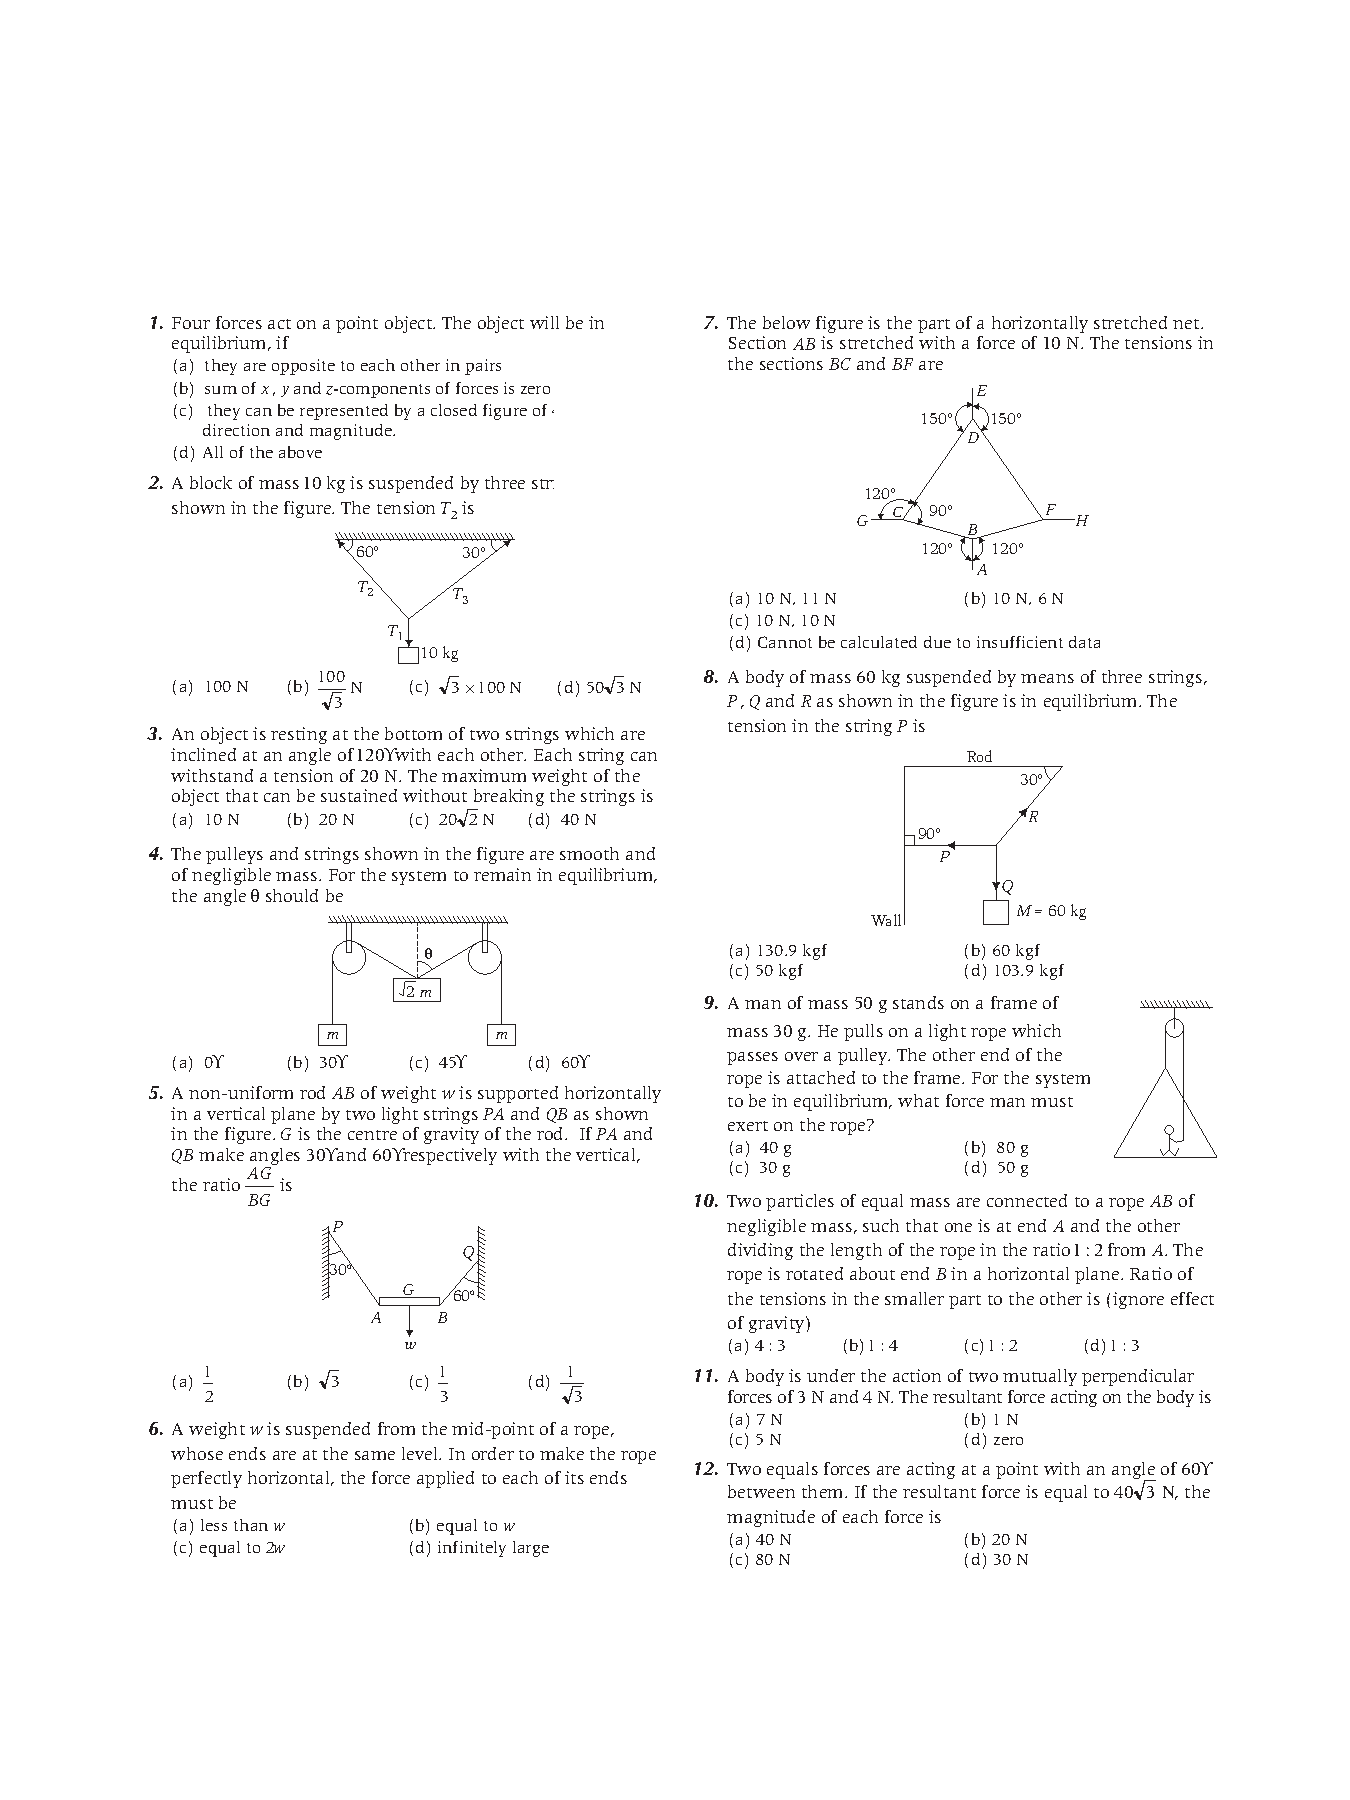
\includegraphics[trim={1cm 0 0 0},clip, width=170 mm]{problem-1-12}
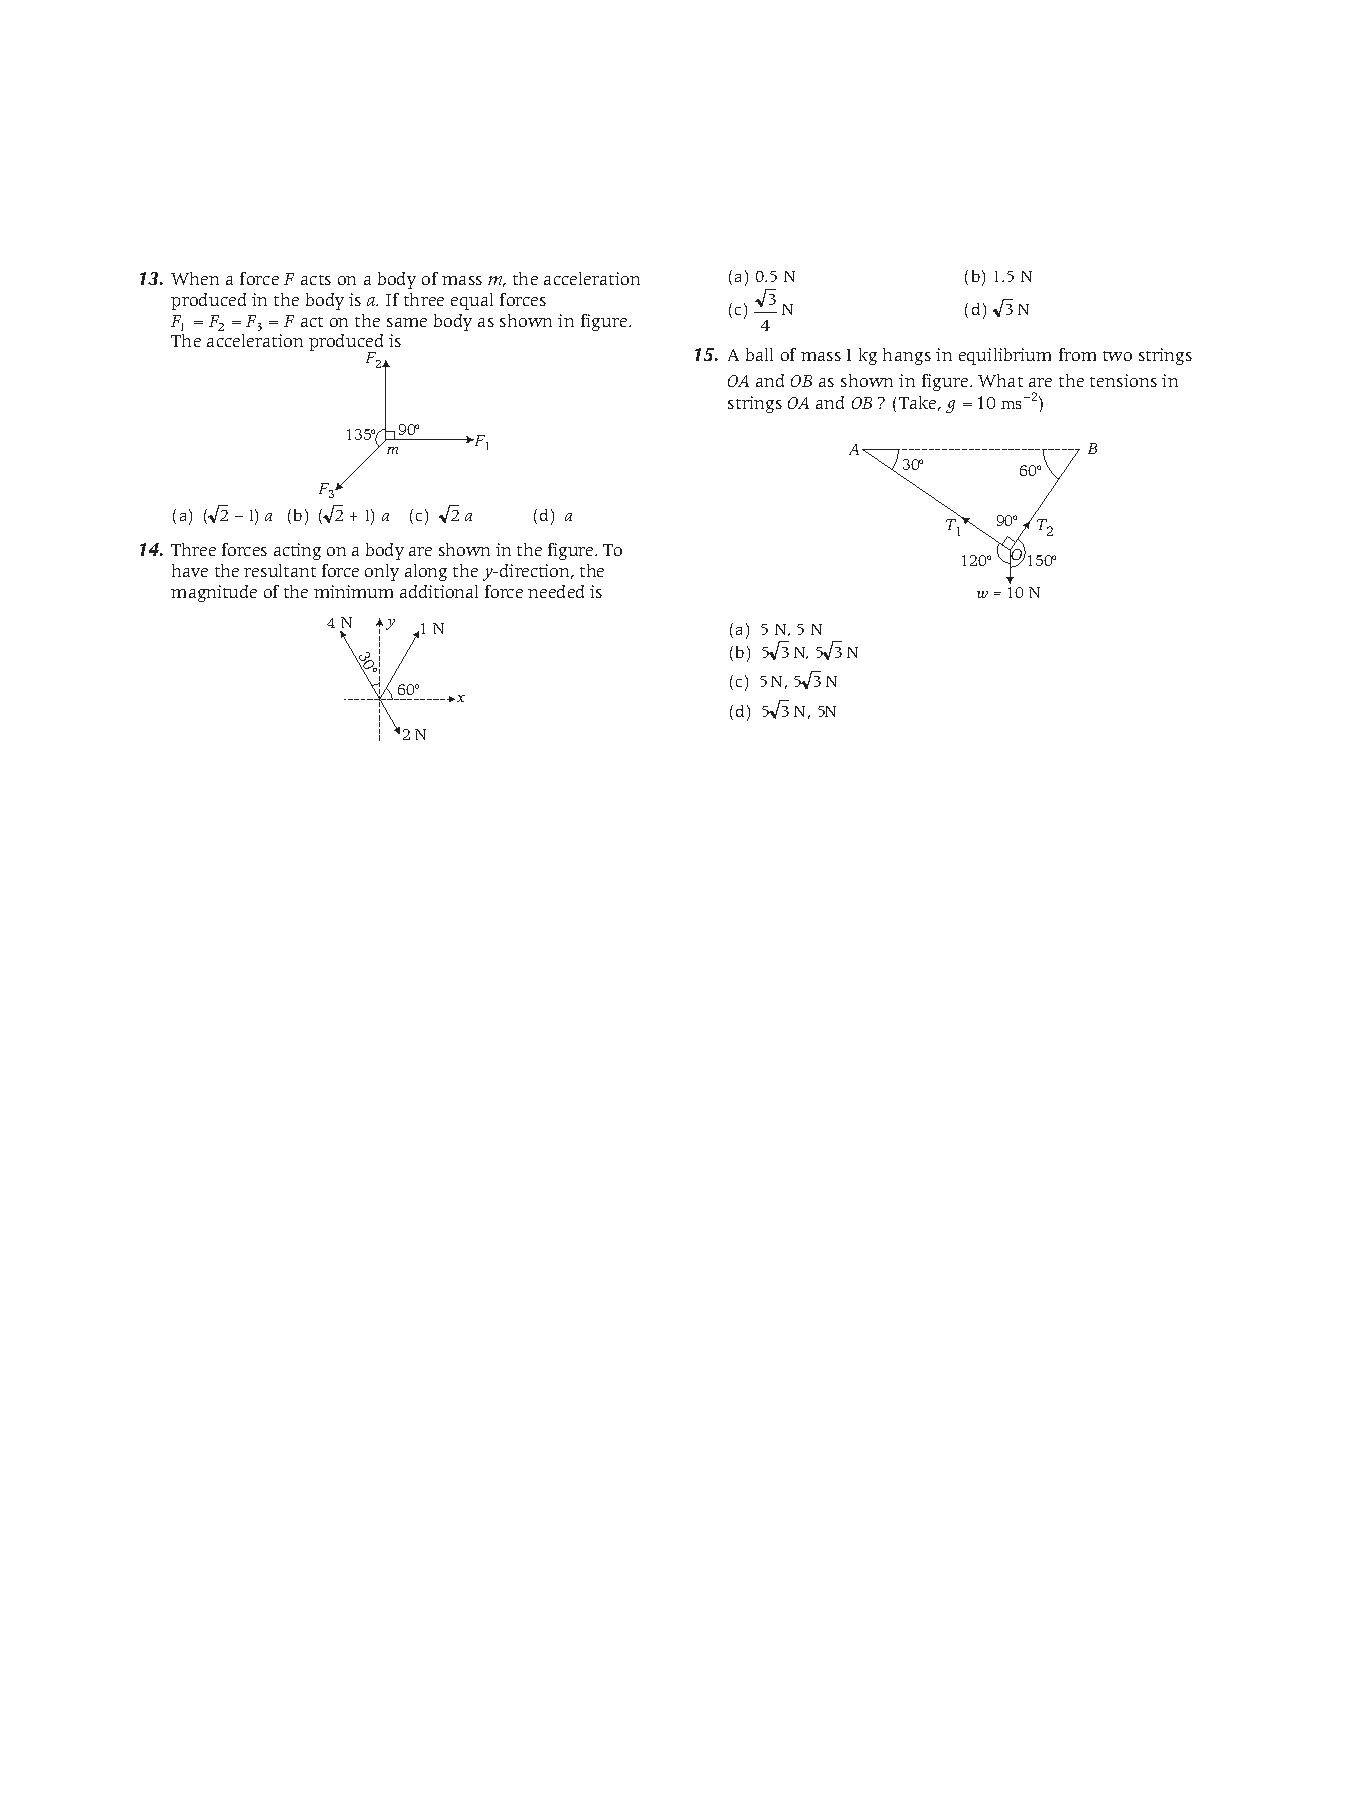
\includegraphics[trim={1cm 0 0 0},clip, width=170 mm]{problem-13-15}
\linebreak
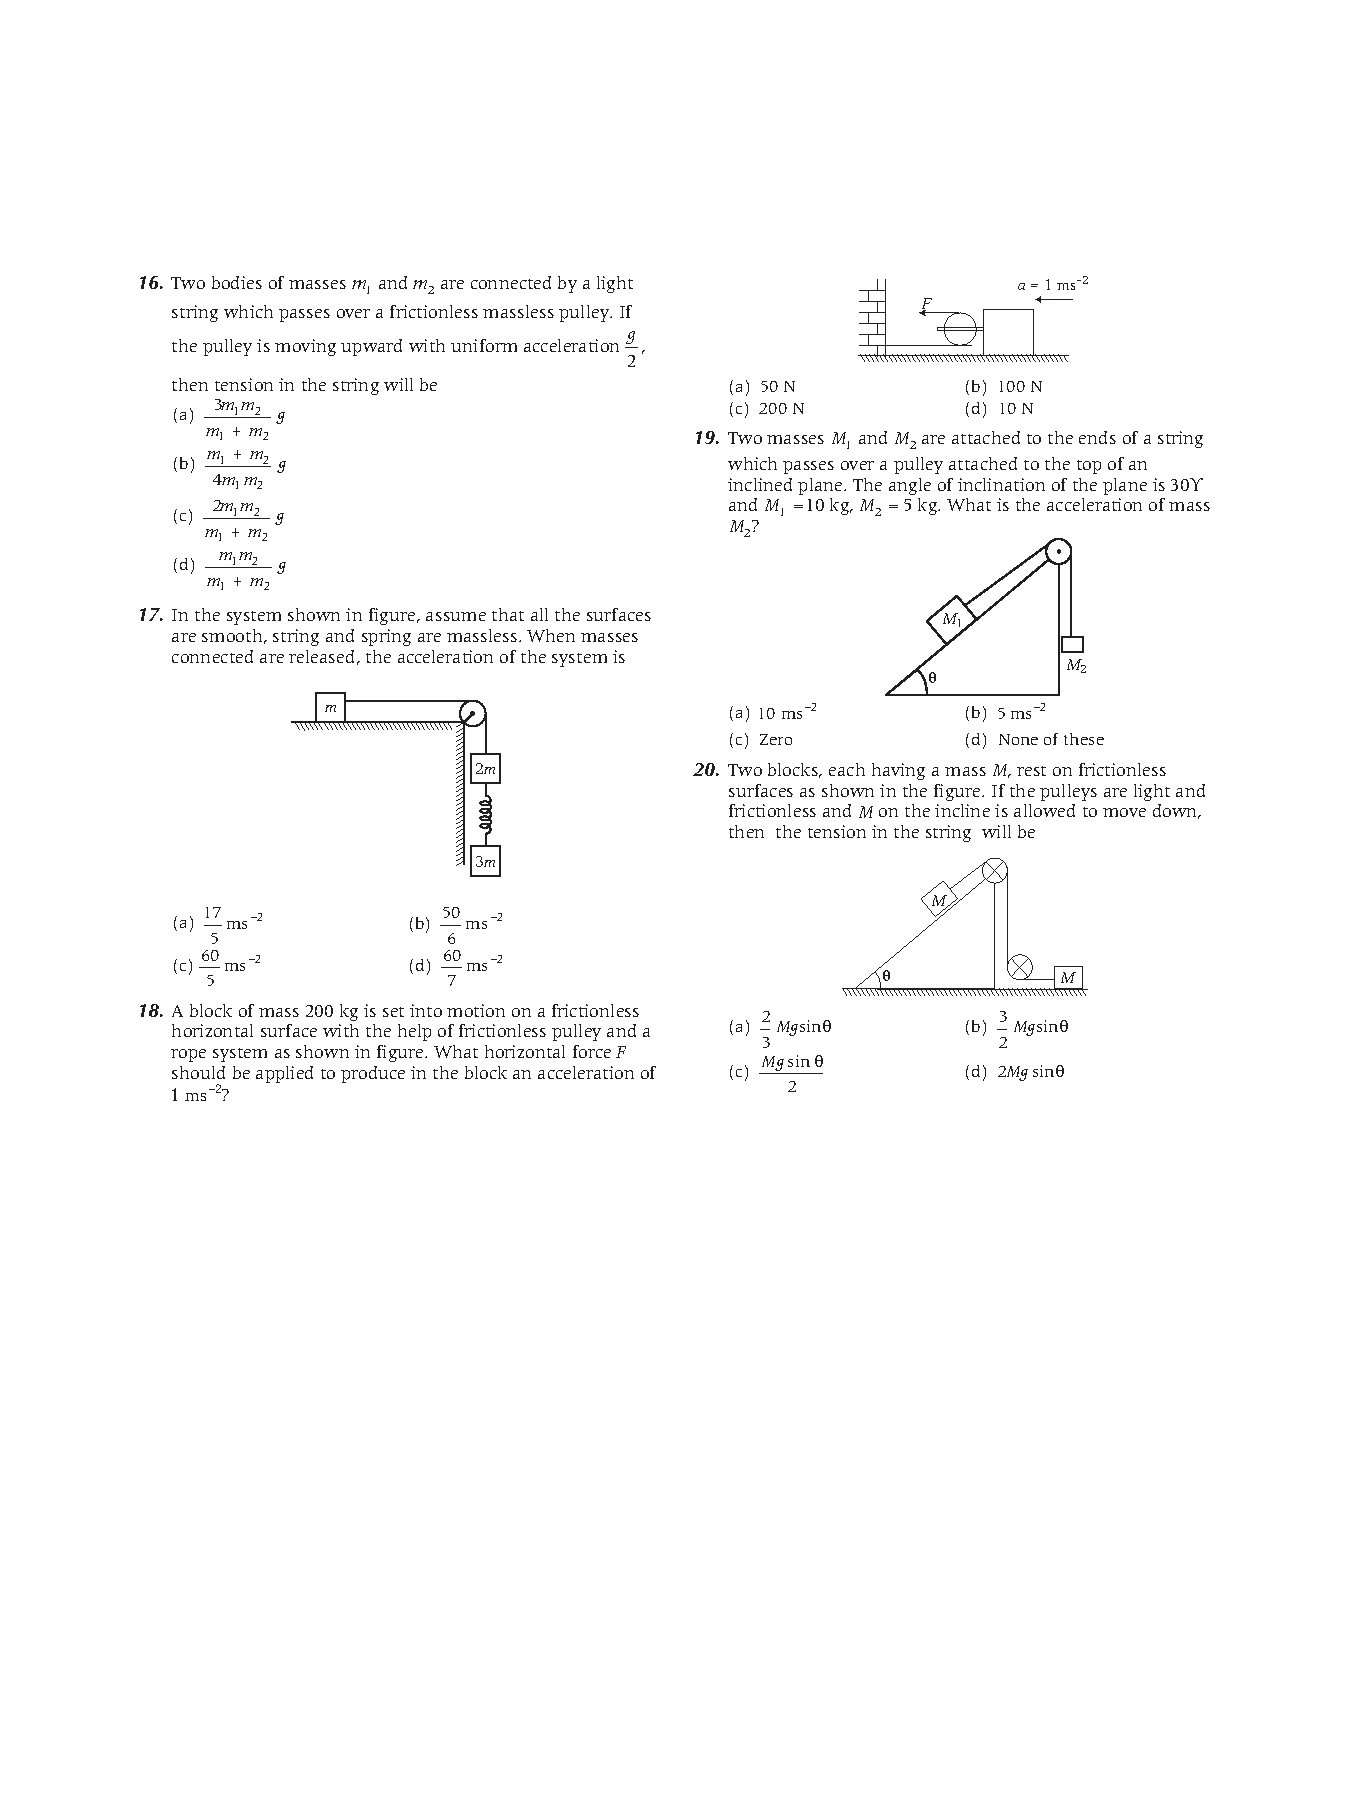
\includegraphics[trim={1cm 0 0 0},clip, width=170 mm]{problem-16-20}



\begin{center}
\textbf{Section-B\\(Numerical Answer Type)}

{\flushleft{This section contains 10 questions. The answer to each question is a NUMERICAL VALUE. For each question, enter the correct numerical value (in decimal notation, truncated/rounded-off to the second decimal place).}}\\

\textbf{Do any 5 questions out of 10 Questions.}

\rule{\textwidth}{1 pt}
\end{center}




\begin{enumerate}
\item A mass of $10 \kg$ is suspended vertically by a rope from the roof. When a horizontal force is applied on the mass, the rope deviated at an angle of $45^\circ$ at the roof point. If the suspended mass is at equilibrium, the magnitude of the force applied in newton is ($g=10\mpss$)\ansit{100}

\item A body of mass $m=10^{-2}\kg$ is moving in a medium and experiences a frictional force $F = -kv^2$. Its initial speed is $v_0 =10\mps$. If,
after $10\s$, its  energy is $\dfrac{1}{8}mv_0^2$, the value of $1000k$ will be \ansit{1}

\item A ball of mass $0.2 \kg$ is thrown vertically upwards by applying a force by hand. If the hand moves $0.2 \m$ while applying the force and the ball goes upto $2 \m$ height further, find the magnitude of the force in newton. \ansit{22}

\item A player caught a cricket ball of mass $150 \gm$ moving at a rate of $20 \mps$. If the catching process is completed in $0.1 \s$, the force of the blow exerted by the ball on the hand of the player is equal to \ansit{30}

\item A block rests on a rough inclined plane making an angle of $30^\circ$ with the horizontal. The coefficient of static friction between the block and the plane is $0.8$. If the frictional force on the block is $10 \N$, the mass of the block (in $\kg$) is ( $g = 10 \mpss$)\ansit{2}

\item A spring balance is attached to the ceiling of a lift. A man hangs his bag on the spring and the spring reads $49 \N$, when the lift is stationary. If the lift moves downward with an acceleration of $5 \mpss$, the reading of the spring balance will be \ansit{24}

\item A block is placed on a rough horizontal surface then the frictional force on the block is \ansit{0}

\item A marble block of mass $2 \kg$ lying on ice when given a velocity of $6 \mps$ is stopped by friction in $10 \s$. Then, the coefficient of friction multiplied by $100$ is \ansit{6}

\item A horizontal force of $10 \N$ is necessary to just
hold a block stationary against a wall. The
coefficient of friction between the block and
the wall is $0.2$. The weight of the block is \ansit{2}

\item Two blocks of equal mass are slacked on top of each other on a horizontal plane, then the frictional force between them is \ansit{0}
\end{enumerate}

\pagebreak

\begin{center}
\texttt{A.N.S.W.E.R.}
\end{center}

\begin{center}
\textbf{Section-A}
\end{center}
\begin{tasks}[label=\arabic*.](2)
	\task (d)
	\task (d)
	\task (b)
	\task (c)
	\task (c)
	\task (d)
	\task (c)
	\task (d)
	\task (a)
	\task (d)
	\task (c)
	\task (a)
	\task (a)
	\task (a)
	\task (c)
	\task (a)
	\task (b)
	\task (b)
	\task (c)
	\task (c)
\end{tasks}

\begin{center}
\textbf{Section-B}
\end{center}
\begin{tasks}[label=\arabic*.](2)
	\task $100$
	\task $1$
	\task $22$
	\task $30$
	\task $2$
	\task $24$
	\task $0$
	\task $6$
	\task $2$
	\task $0$
\end{tasks}



\end{document}
